% Options for packages loaded elsewhere
\PassOptionsToPackage{unicode}{hyperref}
\PassOptionsToPackage{hyphens}{url}
%
\documentclass[
  letterpaper,
  oneside]{scrbook}

\usepackage{amsmath,amssymb}
\usepackage{lmodern}
\usepackage{iftex}
\ifPDFTeX
  \usepackage[T1]{fontenc}
  \usepackage[utf8]{inputenc}
  \usepackage{textcomp} % provide euro and other symbols
\else % if luatex or xetex
  \usepackage{unicode-math}
  \defaultfontfeatures{Scale=MatchLowercase}
  \defaultfontfeatures[\rmfamily]{Ligatures=TeX,Scale=1}
\fi
% Use upquote if available, for straight quotes in verbatim environments
\IfFileExists{upquote.sty}{\usepackage{upquote}}{}
\IfFileExists{microtype.sty}{% use microtype if available
  \usepackage[]{microtype}
  \UseMicrotypeSet[protrusion]{basicmath} % disable protrusion for tt fonts
}{}
\makeatletter
\@ifundefined{KOMAClassName}{% if non-KOMA class
  \IfFileExists{parskip.sty}{%
    \usepackage{parskip}
  }{% else
    \setlength{\parindent}{0pt}
    \setlength{\parskip}{6pt plus 2pt minus 1pt}}
}{% if KOMA class
  \KOMAoptions{parskip=half}}
\makeatother
\usepackage{xcolor}
\usepackage[a4paper]{geometry}
\setlength{\emergencystretch}{3em} % prevent overfull lines
\setcounter{secnumdepth}{5}
% Make \paragraph and \subparagraph free-standing
\ifx\paragraph\undefined\else
  \let\oldparagraph\paragraph
  \renewcommand{\paragraph}[1]{\oldparagraph{#1}\mbox{}}
\fi
\ifx\subparagraph\undefined\else
  \let\oldsubparagraph\subparagraph
  \renewcommand{\subparagraph}[1]{\oldsubparagraph{#1}\mbox{}}
\fi

\usepackage{color}
\usepackage{fancyvrb}
\newcommand{\VerbBar}{|}
\newcommand{\VERB}{\Verb[commandchars=\\\{\}]}
\DefineVerbatimEnvironment{Highlighting}{Verbatim}{commandchars=\\\{\}}
% Add ',fontsize=\small' for more characters per line
\usepackage{framed}
\definecolor{shadecolor}{RGB}{241,243,245}
\newenvironment{Shaded}{\begin{snugshade}}{\end{snugshade}}
\newcommand{\AlertTok}[1]{\textcolor[rgb]{0.68,0.00,0.00}{#1}}
\newcommand{\AnnotationTok}[1]{\textcolor[rgb]{0.37,0.37,0.37}{#1}}
\newcommand{\AttributeTok}[1]{\textcolor[rgb]{0.40,0.45,0.13}{#1}}
\newcommand{\BaseNTok}[1]{\textcolor[rgb]{0.68,0.00,0.00}{#1}}
\newcommand{\BuiltInTok}[1]{\textcolor[rgb]{0.00,0.23,0.31}{#1}}
\newcommand{\CharTok}[1]{\textcolor[rgb]{0.13,0.47,0.30}{#1}}
\newcommand{\CommentTok}[1]{\textcolor[rgb]{0.37,0.37,0.37}{#1}}
\newcommand{\CommentVarTok}[1]{\textcolor[rgb]{0.37,0.37,0.37}{\textit{#1}}}
\newcommand{\ConstantTok}[1]{\textcolor[rgb]{0.56,0.35,0.01}{#1}}
\newcommand{\ControlFlowTok}[1]{\textcolor[rgb]{0.00,0.23,0.31}{#1}}
\newcommand{\DataTypeTok}[1]{\textcolor[rgb]{0.68,0.00,0.00}{#1}}
\newcommand{\DecValTok}[1]{\textcolor[rgb]{0.68,0.00,0.00}{#1}}
\newcommand{\DocumentationTok}[1]{\textcolor[rgb]{0.37,0.37,0.37}{\textit{#1}}}
\newcommand{\ErrorTok}[1]{\textcolor[rgb]{0.68,0.00,0.00}{#1}}
\newcommand{\ExtensionTok}[1]{\textcolor[rgb]{0.00,0.23,0.31}{#1}}
\newcommand{\FloatTok}[1]{\textcolor[rgb]{0.68,0.00,0.00}{#1}}
\newcommand{\FunctionTok}[1]{\textcolor[rgb]{0.28,0.35,0.67}{#1}}
\newcommand{\ImportTok}[1]{\textcolor[rgb]{0.00,0.46,0.62}{#1}}
\newcommand{\InformationTok}[1]{\textcolor[rgb]{0.37,0.37,0.37}{#1}}
\newcommand{\KeywordTok}[1]{\textcolor[rgb]{0.00,0.23,0.31}{#1}}
\newcommand{\NormalTok}[1]{\textcolor[rgb]{0.00,0.23,0.31}{#1}}
\newcommand{\OperatorTok}[1]{\textcolor[rgb]{0.37,0.37,0.37}{#1}}
\newcommand{\OtherTok}[1]{\textcolor[rgb]{0.00,0.23,0.31}{#1}}
\newcommand{\PreprocessorTok}[1]{\textcolor[rgb]{0.68,0.00,0.00}{#1}}
\newcommand{\RegionMarkerTok}[1]{\textcolor[rgb]{0.00,0.23,0.31}{#1}}
\newcommand{\SpecialCharTok}[1]{\textcolor[rgb]{0.37,0.37,0.37}{#1}}
\newcommand{\SpecialStringTok}[1]{\textcolor[rgb]{0.13,0.47,0.30}{#1}}
\newcommand{\StringTok}[1]{\textcolor[rgb]{0.13,0.47,0.30}{#1}}
\newcommand{\VariableTok}[1]{\textcolor[rgb]{0.07,0.07,0.07}{#1}}
\newcommand{\VerbatimStringTok}[1]{\textcolor[rgb]{0.13,0.47,0.30}{#1}}
\newcommand{\WarningTok}[1]{\textcolor[rgb]{0.37,0.37,0.37}{\textit{#1}}}

\providecommand{\tightlist}{%
  \setlength{\itemsep}{0pt}\setlength{\parskip}{0pt}}\usepackage{longtable,booktabs,array}
\usepackage{calc} % for calculating minipage widths
% Correct order of tables after \paragraph or \subparagraph
\usepackage{etoolbox}
\makeatletter
\patchcmd\longtable{\par}{\if@noskipsec\mbox{}\fi\par}{}{}
\makeatother
% Allow footnotes in longtable head/foot
\IfFileExists{footnotehyper.sty}{\usepackage{footnotehyper}}{\usepackage{footnote}}
\makesavenoteenv{longtable}
\usepackage{graphicx}
\makeatletter
\def\maxwidth{\ifdim\Gin@nat@width>\linewidth\linewidth\else\Gin@nat@width\fi}
\def\maxheight{\ifdim\Gin@nat@height>\textheight\textheight\else\Gin@nat@height\fi}
\makeatother
% Scale images if necessary, so that they will not overflow the page
% margins by default, and it is still possible to overwrite the defaults
% using explicit options in \includegraphics[width, height, ...]{}
\setkeys{Gin}{width=\maxwidth,height=\maxheight,keepaspectratio}
% Set default figure placement to htbp
\makeatletter
\def\fps@figure{htbp}
\makeatother
\newlength{\cslhangindent}
\setlength{\cslhangindent}{1.5em}
\newlength{\csllabelwidth}
\setlength{\csllabelwidth}{3em}
\newlength{\cslentryspacingunit} % times entry-spacing
\setlength{\cslentryspacingunit}{\parskip}
\newenvironment{CSLReferences}[2] % #1 hanging-ident, #2 entry spacing
 {% don't indent paragraphs
  \setlength{\parindent}{0pt}
  % turn on hanging indent if param 1 is 1
  \ifodd #1
  \let\oldpar\par
  \def\par{\hangindent=\cslhangindent\oldpar}
  \fi
  % set entry spacing
  \setlength{\parskip}{#2\cslentryspacingunit}
 }%
 {}
\usepackage{calc}
\newcommand{\CSLBlock}[1]{#1\hfill\break}
\newcommand{\CSLLeftMargin}[1]{\parbox[t]{\csllabelwidth}{#1}}
\newcommand{\CSLRightInline}[1]{\parbox[t]{\linewidth - \csllabelwidth}{#1}\break}
\newcommand{\CSLIndent}[1]{\hspace{\cslhangindent}#1}

\newcommand*{\plogo}{\fbox{$\mathcal{PL}$}} % Generic dummy publisher logo
\usepackage[utf8]{inputenc} % Required for inputting international characters
\usepackage[T1]{fontenc} % Output font encoding for international characters
\usepackage{hyphenat}
\usepackage{authblk}

% for nicer tables
\usepackage{booktabs}
\usepackage{longtable}
\usepackage{array}
\usepackage{multirow}
\usepackage{wrapfig}
\usepackage{float}
\usepackage{colortbl}
\usepackage{pdflscape}
\usepackage{tabu}
\usepackage{threeparttable}
\usepackage{threeparttablex}
\usepackage[normalem]{ulem}
\usepackage{makecell}
\usepackage{xcolor}
\usepackage{booktabs}
\usepackage{longtable}
\usepackage{array}
\usepackage{multirow}
\usepackage{wrapfig}
\usepackage{float}
\usepackage{colortbl}
\usepackage{pdflscape}
\usepackage{tabu}
\usepackage{threeparttable}
\usepackage{threeparttablex}
\usepackage[normalem]{ulem}
\usepackage{makecell}
\usepackage{xcolor}
\usepackage{fontspec}
\usepackage{multicol}
\usepackage{hhline}
\newlength\Oldarrayrulewidth
\newlength\Oldtabcolsep
\usepackage{hyperref}
\usepackage{amsmath}
\usepackage{caption}
\makeatletter
\makeatother
\makeatletter
\@ifpackageloaded{bookmark}{}{\usepackage{bookmark}}
\makeatother
\makeatletter
\@ifpackageloaded{caption}{}{\usepackage{caption}}
\AtBeginDocument{%
\ifdefined\contentsname
  \renewcommand*\contentsname{Table of contents}
\else
  \newcommand\contentsname{Table of contents}
\fi
\ifdefined\listfigurename
  \renewcommand*\listfigurename{List of Figures}
\else
  \newcommand\listfigurename{List of Figures}
\fi
\ifdefined\listtablename
  \renewcommand*\listtablename{List of Tables}
\else
  \newcommand\listtablename{List of Tables}
\fi
\ifdefined\figurename
  \renewcommand*\figurename{Figure}
\else
  \newcommand\figurename{Figure}
\fi
\ifdefined\tablename
  \renewcommand*\tablename{Table}
\else
  \newcommand\tablename{Table}
\fi
}
\@ifpackageloaded{float}{}{\usepackage{float}}
\floatstyle{ruled}
\@ifundefined{c@chapter}{\newfloat{codelisting}{h}{lop}}{\newfloat{codelisting}{h}{lop}[chapter]}
\floatname{codelisting}{Listing}
\newcommand*\listoflistings{\listof{codelisting}{List of Listings}}
\makeatother
\makeatletter
\@ifpackageloaded{caption}{}{\usepackage{caption}}
\@ifpackageloaded{subcaption}{}{\usepackage{subcaption}}
\makeatother
\makeatletter
\@ifpackageloaded{tcolorbox}{}{\usepackage[many]{tcolorbox}}
\makeatother
\makeatletter
\@ifundefined{shadecolor}{\definecolor{shadecolor}{rgb}{.97, .97, .97}}
\makeatother
\makeatletter
\makeatother
\ifLuaTeX
  \usepackage{selnolig}  % disable illegal ligatures
\fi
\IfFileExists{bookmark.sty}{\usepackage{bookmark}}{\usepackage{hyperref}}
\IfFileExists{xurl.sty}{\usepackage{xurl}}{} % add URL line breaks if available
\urlstyle{same} % disable monospaced font for URLs
\hypersetup{
  pdftitle={A Quarto Template Repo to Create Big Reports and Very Long Title Because Long Titles are Common},
  pdfauthor={Jane Doe; Eva Nováková; Matti Meikäläinen},
  hidelinks,
  pdfcreator={LaTeX via pandoc}}

\title{A Quarto Template Repo to Create Big Reports and Very Long Title
Because Long Titles are Common}
\usepackage{etoolbox}
\makeatletter
\providecommand{\subtitle}[1]{% add subtitle to \maketitle
  \apptocmd{\@title}{\par {\large #1 \par}}{}{}
}
\makeatother
\subtitle{Some tips on creating reports with Quarto with a focus on
tables and replicated tables and figures}
\author{Jane Doe \and Eva Nováková \and Matti Meikäläinen}
\date{}

\begin{document}


\begin{frontmatter}

	\raggedleft % Right align the title page
	
	\rule{1pt}{\textheight} % Vertical line
	\hspace{0.05\textwidth} % Whitespace between the vertical line and title page text
	\parbox[b]{0.85\textwidth}{ % Paragraph box for holding the title page text, adjust the width to move the title page left or right on the page
	
		{\large\bfseries\nohyphens{A Quarto Template Repo to Create Big Reports
and Very Long Title Because Long Titles are
Common}}\\[2\baselineskip] % Title
				{\large\textit{Some tips on creating reports with Quarto with a focus on
tables and replicated tables and
figures}}\\[4\baselineskip] % Subtitle or further description
				
		        {\large{Jane Doe}}, 
        {\large{Eva Nováková}}        {and \large{Matti Meikäläinen}}
        		
		\vspace{0.5\textheight} % Whitespace between the title block and the publisher
		
		{\noindent The Publisher~~\plogo}\\[\baselineskip] % Publisher and logo
	}

\end{frontmatter}\ifdefined\Shaded\renewenvironment{Shaded}{\begin{tcolorbox}[sharp corners, enhanced, borderline west={3pt}{0pt}{shadecolor}, breakable, frame hidden, boxrule=0pt, interior hidden]}{\end{tcolorbox}}\fi

\renewcommand*\contentsname{Table of contents}
{
\setcounter{tocdepth}{2}
\tableofcontents
}
\listoffigures
\listoftables
\mainmatter
\bookmarksetup{startatroot}

\hypertarget{citation}{%
\chapter*{Citation}\label{citation}}
\addcontentsline{toc}{chapter}{Citation}

\markboth{Citation}{Citation}

EE Holmes, 2022. Quarto Report Template. Northwest Fisheries Science
Center.

\bookmarksetup{startatroot}

\hypertarget{preface}{%
\chapter{Preface}\label{preface}}

Phasellus non diam posuere, laoreet velit sed, egestas felis. Etiam eget
neque in tellus lacinia tincidunt. Pellentesque scelerisque odio velit,
nec fringilla nibh iaculis non. Aenean sit amet nulla ipsum. Cras felis
lacus, pulvinar ac nisi et, convallis pulvinar turpis. Morbi non nibh
lacus. Morbi vitae lorem massa. Sed ut turpis vel felis posuere commodo
lacinia ac mi. Donec finibus lectus sit amet elit finibus, vitae rhoncus
ligula tincidunt. Phasellus vitae blandit lacus. Integer sed nisl
fermentum, pulvinar mauris in, posuere enim. Proin sit amet semper urna.
Vivamus aliquet rutrum diam ac luctus.

\hypertarget{abstract}{%
\section*{Abstract}\label{abstract}}
\addcontentsline{toc}{section}{Abstract}

\markright{Abstract}

Phasellus non diam posuere, laoreet velit sed, egestas felis. Etiam eget
neque in tellus lacinia tincidunt. Pellentesque scelerisque odio velit,
nec fringilla nibh iaculis non. Aenean sit amet nulla ipsum. Cras felis
lacus, pulvinar ac nisi et, convallis pulvinar turpis. Morbi non nibh
lacus. Morbi vitae lorem massa. Sed ut turpis vel felis posuere commodo
lacinia ac mi. Donec finibus lectus sit amet elit finibus, vitae rhoncus
ligula tincidunt. Phasellus vitae blandit lacus. Integer sed nisl
fermentum, pulvinar mauris in, posuere enim. Proin sit amet semper urna.
Vivamus aliquet rutrum diam ac luctus.

\bookmarksetup{startatroot}

\hypertarget{tips}{%
\chapter{Tips}\label{tips}}

\hypertarget{overview}{%
\section{Overview}\label{overview}}

\begin{figure}

{\centering 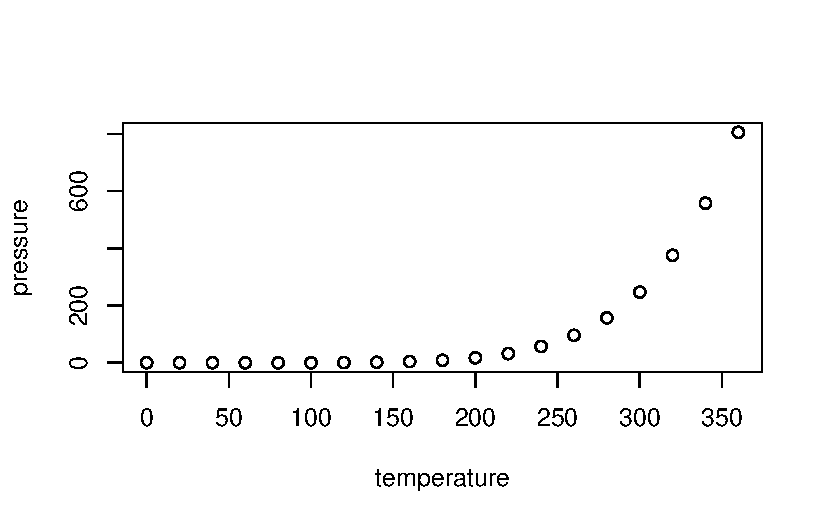
\includegraphics{text/tips_files/figure-pdf/fig-chinook-1.pdf}

}

\caption{\label{fig-chinook}chapter 1 plot}

\end{figure}

\hypertarget{general-set-up}{%
\section{General set-up}\label{general-set-up}}

\begin{itemize}
\item
  Be as modular and simple as you can.
\item
  Don't make everyone in your team be the markdown wizard. You only need
  one person to build the framework.
\item
  Use simple child Rmds so that other team members work only on simple
  Rmd/qmd flat files.
\item
  Don't put all your tables or figures in one huge file:
  \texttt{Table\ xyz.Rmd/qmd}, \texttt{Table\ abc.Rmd/qmd}. Have your
  dedicated markdown wizard figure out the automatic numbering.
\item
  Copy reports built by others who are doing something similar to you.
  TALK within your center or across centers and share work.
\end{itemize}

\hypertarget{tips-1}{%
\section{Tips}\label{tips-1}}

\hypertarget{cross-references}{%
\subsection{Cross-references}\label{cross-references}}

This can be really troublesome unless you use an output that already has
cross-references as part of the design. For R Markdown,

\begin{itemize}
\tightlist
\item
  \{bookdown\} outputs for html and PDF
\item
  \{officedown\} for Word
\end{itemize}

These output formats give you access to cross-referencing via the
\texttt{\textbackslash{}@ref(xxx:yyy)} format and if you use
\texttt{bookdown::pdf\_book}, this will also work with PDF.

However, Quarto makes cross-references, auto-numbering and
cross-referencing of tables and figures super easy.
\href{https://quarto.org/docs/authoring/cross-references.html}{Quarto
cross-ref page}.

For example, we can make a figure with the chunk label \texttt{fig-plot}
like so.

The later in the text we use \texttt{@fig-plot} to get
Figure~\ref{fig-plot}.

\begin{figure}

{\centering 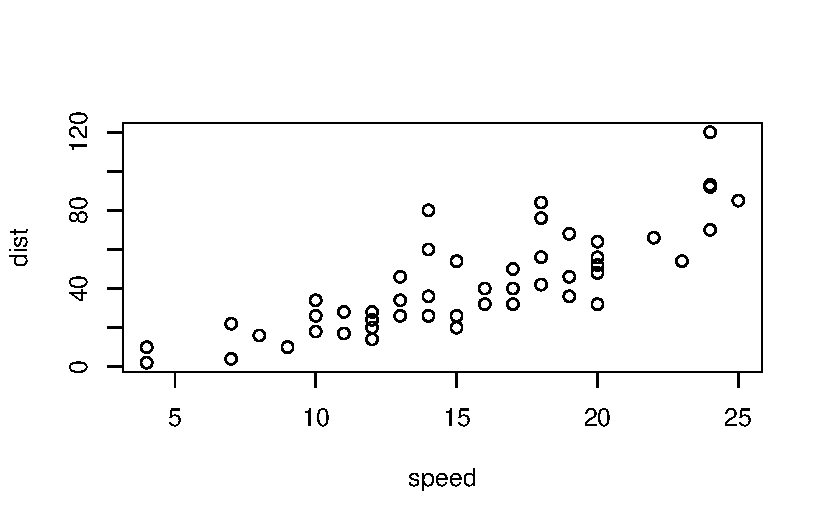
\includegraphics{text/tips_files/figure-pdf/fig-plot-1.pdf}

}

\caption{\label{fig-plot}This is a plot of some data}

\end{figure}

\hypertarget{chunk-labels}{%
\subsection{Chunk labels}\label{chunk-labels}}

\begin{itemize}
\tightlist
\item
  When using R Markdown (or Quarto), it is best not to use chunk labels
  in the your Rmd/qmd children. It's too easy to get duplicate labels
  accidentally.
\end{itemize}

\hypertarget{file-paths}{%
\subsection{File paths}\label{file-paths}}

\begin{itemize}
\tightlist
\item
  if you need to reference a file in a folder, let R create the path so
  that it is compatible across systems:
\end{itemize}

\begin{verbatim}
file.path('figures', 'figure1.Rmd')
\end{verbatim}

\begin{itemize}
\tightlist
\item
  I typically use the \{here\} package so that my code doesn't break if
  I happen to issue a change workspace directory command.
\end{itemize}

\begin{verbatim}
here::here('images', 'logo.png')
\end{verbatim}

\hypertarget{tables-in-for-loops}{%
\subsection{Tables in for loops}\label{tables-in-for-loops}}

Making tables within \texttt{for} loops is tricky and it is different if
you are outputting to Word versus html and also depends on what package
that you use. See my Rmd/qmd files in the tables folder for examples of
how to set it up, but also be prepared for things breaking in the future
as package writers change things. This feature is really fluid. Web
searches on stackoverflow are key for solving these problems.

\hypertarget{working-with-word}{%
\section{Working with Word}\label{working-with-word}}

For many of us, Word is part of our team's workflow. Here are some tips
if that is the case for you:

\begin{itemize}
\tightlist
\item
  Check out the
  \href{https://ardata-fr.github.io/officeverse/index.html}{officeverse}:
  \href{https://CRAN.R-project.org/package=officedown}{officedown} and
  \href{https://CRAN.R-project.org/package=flextable}{flextable} R
  packages.
\item
  Quarto has greatly
  \href{https://quarto.org/docs/output-formats/ms-word.html}{improved
  Word} integration so many of the problems we faced with Word output
  may soon be solved.
\item
  Don't build the whole report in one file. Work on individual text
  sections and then have RStudio (via pandoc/knitr) assemble the report
  (text, figures, tables) from the individual parts.
\item
  How to deal with the team needing to review the assembled document
  (text, figures, tables):

  \begin{itemize}
  \tightlist
  \item
    Try to modularize. So maybe make individual chapters and have review
    happen at that level. Then you incorporate the changes into the
    plain text manually.
  \item
    Use templates to make your Word doc look the way you want. The
    default Word template is bare bones. See my example and read about
    using Word templates with Quartro
    \href{https://quarto.org/docs/output-formats/ms-word-templates.html}{here}
    and R Markdown
    \href{https://bookdown.org/yihui/rmarkdown-cookbook/word-template.html}{here}
    .
  \end{itemize}
\end{itemize}

\hypertarget{making-tables-look-nice-in-word}{%
\subsection{Making tables look nice in
Word}\label{making-tables-look-nice-in-word}}

The example in \texttt{Table\_Counts.Rmd} and
\texttt{Table\_Counts\_flex.Rmd} shows you tricks to make nice Word
tables.

\begin{itemize}
\tightlist
\item
  how to include a page break in your Word doc between tables.
\item
  using \texttt{format="pandoc"} for the table
\item
  using \texttt{results=\textquotesingle{}asis\textquotesingle{}} and
  \texttt{print()} so you can use \texttt{for} loops.
\item
  centering your tables is next to impossible with \texttt{kable()}. Use
  the \{\href{https://ardata-fr.github.io/flextable-book/}{flextable}\}
  package if you need that.
\end{itemize}

\hypertarget{new-pages}{%
\subsection{New pages}\label{new-pages}}

This is how to get a new page in Word. Make sure you are in print view
on the word doc, otherwise you won't see any of the pages.

\begin{verbatim}
```{=openxml}
<w:p><w:r><w:br w:type="page"/></w:r></w:p>
```
\end{verbatim}

\hypertarget{output-templates-with-quarto}{%
\section{Output templates with
Quarto}\label{output-templates-with-quarto}}

Quarto is working on templates to make output to different formats easy.
Here is an example of journal templates
\href{https://github.com/quarto-journals/}{quarto-journals}.

\hypertarget{weird-quarto-quirks}{%
\section{Weird Quarto quirks}\label{weird-quarto-quirks}}

\begin{itemize}
\tightlist
\item
  If you use
\end{itemize}

\begin{verbatim}
---
title: MyTitle
---
\end{verbatim}

as your title spec, then you won't get the first header 2 in your pdf.
Use \texttt{\#} instead.

\begin{itemize}
\item
  If you have 2 \texttt{\#} levels in a qmd file, you only the first
  chapter appearing in the TOC. The others appear weirdly as
  sub-chapters.
\item
  with flextable, your table captions from knitr yaml disappear if the
  table breaks across a page.
\end{itemize}

\bookmarksetup{startatroot}

\hypertarget{tables-intro}{%
\chapter{Tables intro}\label{tables-intro}}

This chapter shows a few simple examples of including tables and getting
cross-referencing to work across formats (HTML, Word, PDF). See
Chapter~\ref{sec-kableflexgt} for more examples and comparisons of
different table outputs.

In this chapter, I am going to use \{flextable\} for Word and HTML and
\{kabelExtra\} for PDF. See Chapter~\ref{sec-kableflexgt} for a
comparison of \{flextable\}, \{kableExtra\} and \{gt\}. There is a
current problem that Quarto is not processing the cross-references with
\{flextable\} into PDF and Word. But this is a known problem and they
are working on it. \{flextable\} is the only table package that I have
found the tends to work as expected across platforms. The \{officer\}
package uses it so it works well with Word and works well with LaTeX.

*Note, I am using some customized functions to be able have a uniform
look for my tables. These are in \texttt{tables/\_common.R}.

\hypertarget{example-table}{%
\section{Example table}\label{example-table}}

This is an example a table. We can reference Table~\ref{tbl-example}
easily and it is auto-numbered.

\hypertarget{tbl-example}{}
\begin{table}
\caption{\label{tbl-example}This is a simple table. }\tabularnewline

\centering
\begin{tabular}[t]{lrrrrrr}
\toprule
  & mpg & cyl & disp & hp & drat & wt\\
\midrule
Mazda RX4 & 21.0 & 6 & 160.0 & 110 & 3.90 & 2.620\\
Mazda RX4 Wag & 21.0 & 6 & 160.0 & 110 & 3.90 & 2.875\\
Datsun 710 & 22.8 & 4 & 108.0 & 93 & 3.85 & 2.320\\
Hornet 4 Drive & 21.4 & 6 & 258.0 & 110 & 3.08 & 3.215\\
Hornet Sportabout & 18.7 & 8 & 360.0 & 175 & 3.15 & 3.440\\
\addlinespace
Valiant & 18.1 & 6 & 225.0 & 105 & 2.76 & 3.460\\
Duster 360 & 14.3 & 8 & 360.0 & 245 & 3.21 & 3.570\\
Merc 240D & 24.4 & 4 & 146.7 & 62 & 3.69 & 3.190\\
Merc 230 & 22.8 & 4 & 140.8 & 95 & 3.92 & 3.150\\
Merc 280 & 19.2 & 6 & 167.6 & 123 & 3.92 & 3.440\\
\bottomrule
\multicolumn{7}{l}{\rule{0pt}{1em}\textit{Note: }}\\
\multicolumn{7}{l}{\rule{0pt}{1em}kable}\\
\end{tabular}
\end{table}

\hypertarget{including-table-files}{%
\section{Including table files}\label{including-table-files}}

It is often good to have your files in separate files so that when you
edit your tables, you only have to work on the table code.

\begin{Shaded}
\begin{Highlighting}[]
\InformationTok{\textasciigrave{}\textasciigrave{}\textasciigrave{}\{r child=here::here("tables", "Table\_flex.Rmd")\}}
\InformationTok{\textasciigrave{}\textasciigrave{}\textasciigrave{}}
\end{Highlighting}
\end{Shaded}

\hypertarget{tbl-flexchild}{}
\global\setlength{\Oldarrayrulewidth}{\arrayrulewidth}

\global\setlength{\Oldtabcolsep}{\tabcolsep}

\setlength{\tabcolsep}{0pt}

\renewcommand*{\arraystretch}{1.5}



\providecommand{\ascline}[3]{\noalign{\global\arrayrulewidth #1}\arrayrulecolor[HTML]{#2}\cline{#3}}

\begin{longtable}[c]{|p{1.34in}|p{0.45in}|p{0.96in}|p{0.95in}|p{1.07in}}

\caption{\label{tbl-flexchild}This table is created in Table\_flex.Rmd. flextable. } \\ 




\multicolumn{1}{>{\raggedright}p{\dimexpr 1.34in+0\tabcolsep}}{\textcolor[HTML]{000000}{\fontsize{11}{11}\selectfont{\textbf{}}}} & \multicolumn{1}{>{\raggedleft}p{\dimexpr 0.45in+0\tabcolsep}}{\textcolor[HTML]{000000}{\fontsize{11}{11}\selectfont{\textbf{Df}}}} & \multicolumn{1}{>{\raggedleft}p{\dimexpr 0.96in+0\tabcolsep}}{\textcolor[HTML]{000000}{\fontsize{11}{11}\selectfont{\textbf{Deviance}}}} & \multicolumn{1}{>{\raggedleft}p{\dimexpr 0.95in+0\tabcolsep}}{\textcolor[HTML]{000000}{\fontsize{11}{11}\selectfont{\textbf{Resid.\ Df}}}} & \multicolumn{1}{>{\raggedleft}p{\dimexpr 1.07in+0\tabcolsep}}{\textcolor[HTML]{000000}{\fontsize{11}{11}\selectfont{\textbf{Resid.\ Dev}}}} \\

\endhead



\multicolumn{1}{>{\raggedright}p{\dimexpr 1.34in+0\tabcolsep}}{\textcolor[HTML]{000000}{\fontsize{12}{12}\selectfont{\textbf{NULL}}}} & \multicolumn{1}{>{\raggedleft}p{\dimexpr 0.45in+0\tabcolsep}}{\textcolor[HTML]{000000}{\fontsize{12}{12}\selectfont{}}} & \multicolumn{1}{>{\raggedleft}p{\dimexpr 0.96in+0\tabcolsep}}{\textcolor[HTML]{000000}{\fontsize{12}{12}\selectfont{}}} & \multicolumn{1}{>{\raggedleft}p{\dimexpr 0.95in+0\tabcolsep}}{\textcolor[HTML]{000000}{\fontsize{12}{12}\selectfont{99}}} & \multicolumn{1}{>{\raggedleft}p{\dimexpr 1.07in+0\tabcolsep}}{\textcolor[HTML]{000000}{\fontsize{12}{12}\selectfont{129.5}}} \\

\ascline{1pt}{000000}{1-5}



\multicolumn{1}{>{\raggedright}p{\dimexpr 1.34in+0\tabcolsep}}{\textcolor[HTML]{000000}{\fontsize{12}{12}\selectfont{\textbf{ethnicty}}}} & \multicolumn{1}{>{\raggedleft}p{\dimexpr 0.45in+0\tabcolsep}}{\textcolor[HTML]{000000}{\fontsize{12}{12}\selectfont{3}}} & \multicolumn{1}{>{\raggedleft}p{\dimexpr 0.96in+0\tabcolsep}}{\textcolor[HTML]{000000}{\fontsize{12}{12}\selectfont{47.2}}} & \multicolumn{1}{>{\raggedleft}p{\dimexpr 0.95in+0\tabcolsep}}{\textcolor[HTML]{000000}{\fontsize{12}{12}\selectfont{96}}} & \multicolumn{1}{>{\raggedleft}p{\dimexpr 1.07in+0\tabcolsep}}{\textcolor[HTML]{000000}{\fontsize{12}{12}\selectfont{82.2}}} \\





\multicolumn{1}{>{\raggedright}p{\dimexpr 1.34in+0\tabcolsep}}{\textcolor[HTML]{000000}{\fontsize{12}{12}\selectfont{\textbf{grade}}}} & \multicolumn{1}{>{\raggedleft}p{\dimexpr 0.45in+0\tabcolsep}}{\textcolor[HTML]{000000}{\fontsize{12}{12}\selectfont{1}}} & \multicolumn{1}{>{\raggedleft}p{\dimexpr 0.96in+0\tabcolsep}}{\textcolor[HTML]{000000}{\fontsize{12}{12}\selectfont{1.7}}} & \multicolumn{1}{>{\raggedleft}p{\dimexpr 0.95in+0\tabcolsep}}{\textcolor[HTML]{000000}{\fontsize{12}{12}\selectfont{95}}} & \multicolumn{1}{>{\raggedleft}p{\dimexpr 1.07in+0\tabcolsep}}{\textcolor[HTML]{000000}{\fontsize{12}{12}\selectfont{80.5}}} \\





\multicolumn{1}{>{\raggedright}p{\dimexpr 1.34in+0\tabcolsep}}{\textcolor[HTML]{000000}{\fontsize{12}{12}\selectfont{\textbf{ethnicty:grade}}}} & \multicolumn{1}{>{\raggedleft}p{\dimexpr 0.45in+0\tabcolsep}}{\textcolor[HTML]{000000}{\fontsize{12}{12}\selectfont{3}}} & \multicolumn{1}{>{\raggedleft}p{\dimexpr 0.96in+0\tabcolsep}}{\textcolor[HTML]{000000}{\fontsize{12}{12}\selectfont{7.2}}} & \multicolumn{1}{>{\raggedleft}p{\dimexpr 0.95in+0\tabcolsep}}{\textcolor[HTML]{000000}{\fontsize{12}{12}\selectfont{92}}} & \multicolumn{1}{>{\raggedleft}p{\dimexpr 1.07in+0\tabcolsep}}{\textcolor[HTML]{000000}{\fontsize{12}{12}\selectfont{73.3}}} \\





\end{longtable}



\arrayrulecolor[HTML]{000000}

\global\setlength{\arrayrulewidth}{\Oldarrayrulewidth}

\global\setlength{\tabcolsep}{\Oldtabcolsep}

\renewcommand*{\arraystretch}{1}

We can add a captions to a flextable with \texttt{set\_caption} but then
we won't have access to Quarto's cross-format (Word, HTML, PDF)
cross-referencing engine. We can also use \texttt{tab.cap="caption"} in
the chunk yaml but again we don't get the cross-referencing engine.

\begin{Shaded}
\begin{Highlighting}[]
\FunctionTok{set\_caption}\NormalTok{(ft, }
  \AttributeTok{caption =} \StringTok{"a table caption with set\_caption"}\NormalTok{, }
  \AttributeTok{style =} \StringTok{"Table Caption"}\NormalTok{)}
\end{Highlighting}
\end{Shaded}

\hypertarget{cross-references-1}{%
\section{Cross-references}\label{cross-references-1}}

In Quarto,
\href{https://quarto.org/docs/authoring/cross-references.html\#tables}{table
links} use the table label \texttt{@tbl-tablabel} where
\texttt{tablabel} is the label you put on the table chunk. In the text
it looks like this Table~\ref{tbl-tablabel}. The chunk yaml looks like
this

\begin{verbatim}
#| label: tbl-tablabel
#| tbl-cap: "my caption"
\end{verbatim}

\hypertarget{tbl-tablabel}{}
\begin{table}
\caption{\label{tbl-tablabel}This is a table with a number. }\tabularnewline

\centering
\begin{tabular}[t]{lrrrrrrrrrrrr}
\toprule
Year & Jan & Feb & Mar & Apr & May & Jun & Jul & Aug & Sep & Oct & Nov & Dec\\
\midrule
1954 & NA & NA & NA & NA & NA & NA & -1 & -1 & 1 & 3 & 5 & 4\\
1955 & 3 & 4 & 4 & 7 & 9 & 11 & 12 & 13 & 17 & 18 & 19 & 19\\
1956 & 19 & 20 & 22 & 22 & 22 & 24 & 24 & 27 & 28 & 29 & 30 & 32\\
1957 & 32 & 33 & 32 & 32 & 33 & 34 & 37 & 37 & 38 & 40 & 41 & 41\\
1958 & 42 & 42 & 43 & 43 & 44 & 43 & 43 & 45 & 46 & 48 & 50 & 52\\
\addlinespace
1959 & 53 & 52 & 54 & 56 & 57 & 59 & 61 & 61 & 61 & 62 & 62 & 62\\
1960 & 62 & 64 & 65 & 66 & 68 & 68 & 69 & 69 & 70 & 71 & 74 & 75\\
1961 & 75 & 77 & 76 & 77 & 77 & 78 & 78 & 78 & 80 & 82 & 83 & 85\\
1962 & 87 & 88 & 86 & 87 & 88 & 90 & 90 & 92 & 92 & 93 & NA & NA\\
\bottomrule
\multicolumn{13}{l}{\rule{0pt}{1em}\textit{Note: }}\\
\multicolumn{13}{l}{\rule{0pt}{1em}kable}\\
\end{tabular}
\end{table}

\hypertarget{dynamic-table-captions}{%
\section{Dynamic table captions}\label{dynamic-table-captions}}

You can create captions dynamically.

\begin{Shaded}
\begin{Highlighting}[]
\NormalTok{dt }\OtherTok{\textless{}{-}}\NormalTok{ mtcars[}\DecValTok{1}\SpecialCharTok{:}\DecValTok{10}\NormalTok{, }\DecValTok{1}\SpecialCharTok{:}\DecValTok{6}\NormalTok{]}
\NormalTok{tbl\_cap }\OtherTok{\textless{}{-}} \FunctionTok{paste}\NormalTok{(}\StringTok{"This is a dynamically created caption. The length of mtcars is"}\NormalTok{, }\FunctionTok{nrow}\NormalTok{(mtcars), }\StringTok{"rows. Here we show"}\NormalTok{, }\FunctionTok{nrow}\NormalTok{(dt), }\StringTok{"rows."}\NormalTok{)}
\end{Highlighting}
\end{Shaded}

Unfortunately you cannot dynamically create your chunk labels too.

\hypertarget{tbl-test3}{}
\begin{table}
\caption{\label{tbl-test3}This is a dynamically created caption. The length of mtcars is 32 rows.
Here we show 10 rows. }\tabularnewline

\centering
\begin{tabular}[t]{lrrrrrr}
\toprule
  & mpg & cyl & disp & hp & drat & wt\\
\midrule
Mazda RX4 & 21.0 & 6 & 160.0 & 110 & 3.90 & 2.620\\
Mazda RX4 Wag & 21.0 & 6 & 160.0 & 110 & 3.90 & 2.875\\
Datsun 710 & 22.8 & 4 & 108.0 & 93 & 3.85 & 2.320\\
Hornet 4 Drive & 21.4 & 6 & 258.0 & 110 & 3.08 & 3.215\\
Hornet Sportabout & 18.7 & 8 & 360.0 & 175 & 3.15 & 3.440\\
\addlinespace
Valiant & 18.1 & 6 & 225.0 & 105 & 2.76 & 3.460\\
Duster 360 & 14.3 & 8 & 360.0 & 245 & 3.21 & 3.570\\
Merc 240D & 24.4 & 4 & 146.7 & 62 & 3.69 & 3.190\\
Merc 230 & 22.8 & 4 & 140.8 & 95 & 3.92 & 3.150\\
Merc 280 & 19.2 & 6 & 167.6 & 123 & 3.92 & 3.440\\
\bottomrule
\multicolumn{7}{l}{\rule{0pt}{1em}\textit{Note: }}\\
\multicolumn{7}{l}{\rule{0pt}{1em}kable}\\
\end{tabular}
\end{table}

\bookmarksetup{startatroot}

\hypertarget{tables-in-a-for-loop}{%
\chapter{Tables in a for loop}\label{tables-in-a-for-loop}}

Outputting tables (or figure) in a for loop works fine in Quarto, but
there is no way to set the table numbers dynamically and get all the
cross-references working in Word, HTML and PDF. We really need that
dynamic numbering and cross-reference feature in a big report.

\hypertarget{example-of-tables-produced-in-a-for-loop}{%
\section{Example of tables produced in a for
loop}\label{example-of-tables-produced-in-a-for-loop}}

Look at the Code (link at top in HTML output) to see the
\texttt{cat(knitr::knit\_print(tab))} trick for getting your tables to
appear.

\begin{table}

\caption{We can set a caption but no way to cross-reference it}
\centering
\begin{tabular}[t]{lrrrr}
\toprule
  & mpg & cyl & disp & hp\\
\midrule
Mazda RX4 & 21 & 6 & 160 & 110\\
Mazda RX4 Wag & 21 & 6 & 160 & 110\\
\bottomrule
\multicolumn{5}{l}{\rule{0pt}{1em}\textit{Note: }}\\
\multicolumn{5}{l}{\rule{0pt}{1em}kable}\\
\end{tabular}
\end{table}

\begin{table}

\caption{We can set a caption but no way to cross-reference it}
\centering
\begin{tabular}[t]{lrrrr}
\toprule
  & mpg & cyl & disp & hp\\
\midrule
Mazda RX4 & 21 & 6 & 160 & 110\\
Mazda RX4 Wag & 21 & 6 & 160 & 110\\
\bottomrule
\multicolumn{5}{l}{\rule{0pt}{1em}\textit{Note: }}\\
\multicolumn{5}{l}{\rule{0pt}{1em}kable}\\
\end{tabular}
\end{table}

\hypertarget{getting-the-cross-reference-links}{%
\section{Getting the cross-reference
links}\label{getting-the-cross-reference-links}}

We have to use a bit of magic to get our dynamic table numbers and links
using Quarto's cross-referencing. The trick is to use a child Rmd (or
qmd) in a for loop. This trick can be used for figures too but I'll just
show it here with tables. This code inspired from
\href{https://gist.github.com/rmoff/a043676a2f084b81a434}{this gist}.

We use \texttt{knit\_expand()} and make a child Rmd that uses double
curly braces like \texttt{\{\{value.to.match\}\}} in the code. That way
the value at the time this Rmd was embedded can be referenced. Note that
if \texttt{value.to.match} were a string (which it is not in this
example), we would need to add quotes around
\texttt{\{\{value.to.match\}\}} in our code.

With this approach we get our numbered tables and we can reference the
tables usual such as Table~\ref{tbl-cyl8}. Click on the Code link at top
(HTML output) to see how it's done.

\hypertarget{tbl-cyl4}{}
\begin{table}
\caption{\label{tbl-cyl4}Cars with 4 cylinders. These tables have cross-ref links via @tbl-xyz. }\tabularnewline

\centering
\begin{tabular}[t]{lrrrr}
\toprule
  & mpg & cyl & disp & hp\\
\midrule
Datsun 710 & 22.8 & 4 & 108.0 & 93\\
Merc 240D & 24.4 & 4 & 146.7 & 62\\
Merc 230 & 22.8 & 4 & 140.8 & 95\\
\bottomrule
\multicolumn{5}{l}{\rule{0pt}{1em}\textit{Note: }}\\
\multicolumn{5}{l}{\rule{0pt}{1em}kable}\\
\end{tabular}
\end{table}

\hypertarget{tbl-cyl8}{}
\begin{table}
\caption{\label{tbl-cyl8}Cars with 8 cylinders. These tables have cross-ref links via @tbl-xyz. }\tabularnewline

\centering
\begin{tabular}[t]{lrrrr}
\toprule
  & mpg & cyl & disp & hp\\
\midrule
Hornet Sportabout & 18.7 & 8 & 360.0 & 175\\
Duster 360 & 14.3 & 8 & 360.0 & 245\\
Merc 450SE & 16.4 & 8 & 275.8 & 180\\
\bottomrule
\multicolumn{5}{l}{\rule{0pt}{1em}\textit{Note: }}\\
\multicolumn{5}{l}{\rule{0pt}{1em}kable}\\
\end{tabular}
\end{table}

\bookmarksetup{startatroot}

\hypertarget{sec-kableflexgt}{%
\chapter{Kable vs Flex vs qt}\label{sec-kableflexgt}}

Here I compare a three different ways to make tables. Unfortunately the
table numbers and cross-references are still not working as of Quarto
version 1.2.335 (Feb 2023), but the developers are aware and a major
revamp of cross-referencing is in the works to fix these problems.

\hypertarget{kable}{%
\section{Kable}\label{kable}}

Here is the \{kable\} table Table~\ref{tbl-kable}. Word output is often
not good looking. This is a known issue with \texttt{kable}.

\begin{Shaded}
\begin{Highlighting}[]
\FunctionTok{library}\NormalTok{(knitr)}
\FunctionTok{library}\NormalTok{(kableExtra)}
\CommentTok{\# note hold\_position not working in Quarto v1.0.38.}
\FunctionTok{kbl}\NormalTok{(dt, }\AttributeTok{booktabs =} \ConstantTok{TRUE}\NormalTok{) }\SpecialCharTok{\%\textgreater{}\%}
  \FunctionTok{kable\_styling}\NormalTok{(}\AttributeTok{latex\_options =} \FunctionTok{c}\NormalTok{(}\StringTok{"scale\_down"}\NormalTok{)) }\SpecialCharTok{\%\textgreater{}\%}
\NormalTok{  kableExtra}\SpecialCharTok{::}\FunctionTok{footnote}\NormalTok{(}\AttributeTok{symbol =} \FunctionTok{c}\NormalTok{(f1, f2))}
\end{Highlighting}
\end{Shaded}

\hypertarget{tbl-kable}{}
\begin{table}
\caption{\label{tbl-kable}kable: This should have a number that follows the other tables. }\tabularnewline

\centering
\resizebox{\linewidth}{!}{
\begin{tabular}[t]{lrrrrrrrrrrr}
\toprule
  & mpg & cyl & disp & hp & drat & wt & qsec & vs & am & gear & carb\\
\midrule
Mazda RX4 & 21.0 & 6 & 160.0 & 110 & 3.90 & 2.620 & 16.46 & 0 & 1 & 4 & 4\\
Mazda RX4 Wag & 21.0 & 6 & 160.0 & 110 & 3.90 & 2.875 & 17.02 & 0 & 1 & 4 & 4\\
Datsun 710 & 22.8 & 4 & 108.0 & 93 & 3.85 & 2.320 & 18.61 & 1 & 1 & 4 & 1\\
Hornet 4 Drive & 21.4 & 6 & 258.0 & 110 & 3.08 & 3.215 & 19.44 & 1 & 0 & 3 & 1\\
Hornet Sportabout & 18.7 & 8 & 360.0 & 175 & 3.15 & 3.440 & 17.02 & 0 & 0 & 3 & 2\\
\addlinespace
Valiant & 18.1 & 6 & 225.0 & 105 & 2.76 & 3.460 & 20.22 & 1 & 0 & 3 & 1\\
Duster 360 & 14.3 & 8 & 360.0 & 245 & 3.21 & 3.570 & 15.84 & 0 & 0 & 3 & 4\\
Merc 240D & 24.4 & 4 & 146.7 & 62 & 3.69 & 3.190 & 20.00 & 1 & 0 & 4 & 2\\
Merc 230 & 22.8 & 4 & 140.8 & 95 & 3.92 & 3.150 & 22.90 & 1 & 0 & 4 & 2\\
Merc 280 & 19.2 & 6 & 167.6 & 123 & 3.92 & 3.440 & 18.30 & 1 & 0 & 4 & 4\\
\bottomrule
\multicolumn{12}{l}{\rule{0pt}{1em}\textsuperscript{*} Here is a footnote about this table}\\
\multicolumn{12}{l}{\rule{0pt}{1em}\textsuperscript{\dag} Here is a second footnote.}\\
\end{tabular}}
\end{table}

\hypertarget{kable-quirks}{%
\subsection{\texorpdfstring{\texttt{kable}
quirks}{kable quirks}}\label{kable-quirks}}

\begin{itemize}
\tightlist
\item
  Make sure to put \texttt{always\_allow\_html:\ true} in the yaml at
  the top of your Rmd or qmd file if outputting to Word. I can't figure
  out how to put it in the `
\item
  Word output is often not good looking. This is a known issue with
  \texttt{kable}
\item
  Do not pass in caption to \texttt{kbl()} if you want to use Quarto's
  cross-reference engine.
\item
  \texttt{kbl(...,\ format="pandoc")} can help for Word if your
  templates stop working but destroys the PDF output.
\end{itemize}

\hypertarget{flextable}{%
\section{\texorpdfstring{\texttt{flextable}}{flextable}}\label{flextable}}

Here is the \{flextable\} table Table~\ref{tbl-flex}. \{flextable\}
gives you a lot more control over your tables with a grammar format
(like ggplot2). It also gives nice output to Word, PDF and HTML. Sadly
in Quarto v1.2.335 cross-reference and table numbers for Word is broken,
but the developers know about this. The \{officer\} package, which I
think Quarto is leaning on for Word generation, use \{flextable\} so I
am hoping that \{flextable\} gets moved into the RStudio suite.

\begin{Shaded}
\begin{Highlighting}[]
\FunctionTok{library}\NormalTok{(flextable)}
\NormalTok{dt }\SpecialCharTok{\%\textgreater{}\%}
  \FunctionTok{flextable}\NormalTok{() }\SpecialCharTok{\%\textgreater{}\%}
  \FunctionTok{autofit}\NormalTok{() }\SpecialCharTok{\%\textgreater{}\%}
\NormalTok{  flextable}\SpecialCharTok{::}\FunctionTok{footnote}\NormalTok{(}\AttributeTok{i =} \DecValTok{1}\NormalTok{, }\AttributeTok{j =} \DecValTok{1}\SpecialCharTok{:}\DecValTok{2}\NormalTok{,}
            \AttributeTok{value =} \FunctionTok{as\_paragraph}\NormalTok{(}\FunctionTok{c}\NormalTok{(f1, f2)),}
            \AttributeTok{ref\_symbols =} \FunctionTok{c}\NormalTok{(}\StringTok{"a"}\NormalTok{, }\StringTok{"b"}\NormalTok{),}
            \AttributeTok{part =} \StringTok{"header"}\NormalTok{) }\SpecialCharTok{\%\textgreater{}\%}
  \FunctionTok{font}\NormalTok{(}\AttributeTok{fontname=}\StringTok{"Times New Roman"}\NormalTok{, }\AttributeTok{part=}\StringTok{"all"}\NormalTok{) }\SpecialCharTok{\%\textgreater{}\%}
  \FunctionTok{fontsize}\NormalTok{(}\AttributeTok{size=}\DecValTok{12}\NormalTok{)}
\end{Highlighting}
\end{Shaded}

\hypertarget{tbl-flex}{}
\global\setlength{\Oldarrayrulewidth}{\arrayrulewidth}

\global\setlength{\Oldtabcolsep}{\tabcolsep}

\setlength{\tabcolsep}{0pt}

\renewcommand*{\arraystretch}{1.5}



\providecommand{\ascline}[3]{\noalign{\global\arrayrulewidth #1}\arrayrulecolor[HTML]{#2}\cline{#3}}

\begin{longtable}[c]{|p{0.58in}|p{0.47in}|p{0.67in}|p{0.54in}|p{0.58in}|p{0.67in}|p{0.67in}|p{0.44in}|p{0.50in}|p{0.59in}|p{0.58in}}

\caption{\label{tbl-flex}flextable: This should have a number that follows the other tables. } \\ 


\ascline{2pt}{666666}{1-11}

\multicolumn{1}{>{\raggedleft}p{\dimexpr 0.58in+0\tabcolsep}}{\textcolor[HTML]{000000}{\fontsize{11}{11}\selectfont{mpg}}\textcolor[HTML]{000000}{\textsuperscript{\fontsize{11}{11}\selectfont{a}}}} & \multicolumn{1}{>{\raggedleft}p{\dimexpr 0.47in+0\tabcolsep}}{\textcolor[HTML]{000000}{\fontsize{11}{11}\selectfont{cyl}}\textcolor[HTML]{000000}{\textsuperscript{\fontsize{11}{11}\selectfont{b}}}} & \multicolumn{1}{>{\raggedleft}p{\dimexpr 0.67in+0\tabcolsep}}{\textcolor[HTML]{000000}{\fontsize{11}{11}\selectfont{disp}}} & \multicolumn{1}{>{\raggedleft}p{\dimexpr 0.54in+0\tabcolsep}}{\textcolor[HTML]{000000}{\fontsize{11}{11}\selectfont{hp}}} & \multicolumn{1}{>{\raggedleft}p{\dimexpr 0.58in+0\tabcolsep}}{\textcolor[HTML]{000000}{\fontsize{11}{11}\selectfont{drat}}} & \multicolumn{1}{>{\raggedleft}p{\dimexpr 0.67in+0\tabcolsep}}{\textcolor[HTML]{000000}{\fontsize{11}{11}\selectfont{wt}}} & \multicolumn{1}{>{\raggedleft}p{\dimexpr 0.67in+0\tabcolsep}}{\textcolor[HTML]{000000}{\fontsize{11}{11}\selectfont{qsec}}} & \multicolumn{1}{>{\raggedleft}p{\dimexpr 0.44in+0\tabcolsep}}{\textcolor[HTML]{000000}{\fontsize{11}{11}\selectfont{vs}}} & \multicolumn{1}{>{\raggedleft}p{\dimexpr 0.5in+0\tabcolsep}}{\textcolor[HTML]{000000}{\fontsize{11}{11}\selectfont{am}}} & \multicolumn{1}{>{\raggedleft}p{\dimexpr 0.59in+0\tabcolsep}}{\textcolor[HTML]{000000}{\fontsize{11}{11}\selectfont{gear}}} & \multicolumn{1}{>{\raggedleft}p{\dimexpr 0.58in+0\tabcolsep}}{\textcolor[HTML]{000000}{\fontsize{11}{11}\selectfont{carb}}} \\

\ascline{2pt}{666666}{1-11}\endhead



\multicolumn{1}{>{\raggedleft}p{\dimexpr 0.58in+0\tabcolsep}}{\textcolor[HTML]{000000}{\fontsize{12}{12}\selectfont{21.0}}} & \multicolumn{1}{>{\raggedleft}p{\dimexpr 0.47in+0\tabcolsep}}{\textcolor[HTML]{000000}{\fontsize{12}{12}\selectfont{6}}} & \multicolumn{1}{>{\raggedleft}p{\dimexpr 0.67in+0\tabcolsep}}{\textcolor[HTML]{000000}{\fontsize{12}{12}\selectfont{160.0}}} & \multicolumn{1}{>{\raggedleft}p{\dimexpr 0.54in+0\tabcolsep}}{\textcolor[HTML]{000000}{\fontsize{12}{12}\selectfont{110}}} & \multicolumn{1}{>{\raggedleft}p{\dimexpr 0.58in+0\tabcolsep}}{\textcolor[HTML]{000000}{\fontsize{12}{12}\selectfont{3.90}}} & \multicolumn{1}{>{\raggedleft}p{\dimexpr 0.67in+0\tabcolsep}}{\textcolor[HTML]{000000}{\fontsize{12}{12}\selectfont{2.620}}} & \multicolumn{1}{>{\raggedleft}p{\dimexpr 0.67in+0\tabcolsep}}{\textcolor[HTML]{000000}{\fontsize{12}{12}\selectfont{16.46}}} & \multicolumn{1}{>{\raggedleft}p{\dimexpr 0.44in+0\tabcolsep}}{\textcolor[HTML]{000000}{\fontsize{12}{12}\selectfont{0}}} & \multicolumn{1}{>{\raggedleft}p{\dimexpr 0.5in+0\tabcolsep}}{\textcolor[HTML]{000000}{\fontsize{12}{12}\selectfont{1}}} & \multicolumn{1}{>{\raggedleft}p{\dimexpr 0.59in+0\tabcolsep}}{\textcolor[HTML]{000000}{\fontsize{12}{12}\selectfont{4}}} & \multicolumn{1}{>{\raggedleft}p{\dimexpr 0.58in+0\tabcolsep}}{\textcolor[HTML]{000000}{\fontsize{12}{12}\selectfont{4}}} \\





\multicolumn{1}{>{\raggedleft}p{\dimexpr 0.58in+0\tabcolsep}}{\textcolor[HTML]{000000}{\fontsize{12}{12}\selectfont{21.0}}} & \multicolumn{1}{>{\raggedleft}p{\dimexpr 0.47in+0\tabcolsep}}{\textcolor[HTML]{000000}{\fontsize{12}{12}\selectfont{6}}} & \multicolumn{1}{>{\raggedleft}p{\dimexpr 0.67in+0\tabcolsep}}{\textcolor[HTML]{000000}{\fontsize{12}{12}\selectfont{160.0}}} & \multicolumn{1}{>{\raggedleft}p{\dimexpr 0.54in+0\tabcolsep}}{\textcolor[HTML]{000000}{\fontsize{12}{12}\selectfont{110}}} & \multicolumn{1}{>{\raggedleft}p{\dimexpr 0.58in+0\tabcolsep}}{\textcolor[HTML]{000000}{\fontsize{12}{12}\selectfont{3.90}}} & \multicolumn{1}{>{\raggedleft}p{\dimexpr 0.67in+0\tabcolsep}}{\textcolor[HTML]{000000}{\fontsize{12}{12}\selectfont{2.875}}} & \multicolumn{1}{>{\raggedleft}p{\dimexpr 0.67in+0\tabcolsep}}{\textcolor[HTML]{000000}{\fontsize{12}{12}\selectfont{17.02}}} & \multicolumn{1}{>{\raggedleft}p{\dimexpr 0.44in+0\tabcolsep}}{\textcolor[HTML]{000000}{\fontsize{12}{12}\selectfont{0}}} & \multicolumn{1}{>{\raggedleft}p{\dimexpr 0.5in+0\tabcolsep}}{\textcolor[HTML]{000000}{\fontsize{12}{12}\selectfont{1}}} & \multicolumn{1}{>{\raggedleft}p{\dimexpr 0.59in+0\tabcolsep}}{\textcolor[HTML]{000000}{\fontsize{12}{12}\selectfont{4}}} & \multicolumn{1}{>{\raggedleft}p{\dimexpr 0.58in+0\tabcolsep}}{\textcolor[HTML]{000000}{\fontsize{12}{12}\selectfont{4}}} \\





\multicolumn{1}{>{\raggedleft}p{\dimexpr 0.58in+0\tabcolsep}}{\textcolor[HTML]{000000}{\fontsize{12}{12}\selectfont{22.8}}} & \multicolumn{1}{>{\raggedleft}p{\dimexpr 0.47in+0\tabcolsep}}{\textcolor[HTML]{000000}{\fontsize{12}{12}\selectfont{4}}} & \multicolumn{1}{>{\raggedleft}p{\dimexpr 0.67in+0\tabcolsep}}{\textcolor[HTML]{000000}{\fontsize{12}{12}\selectfont{108.0}}} & \multicolumn{1}{>{\raggedleft}p{\dimexpr 0.54in+0\tabcolsep}}{\textcolor[HTML]{000000}{\fontsize{12}{12}\selectfont{93}}} & \multicolumn{1}{>{\raggedleft}p{\dimexpr 0.58in+0\tabcolsep}}{\textcolor[HTML]{000000}{\fontsize{12}{12}\selectfont{3.85}}} & \multicolumn{1}{>{\raggedleft}p{\dimexpr 0.67in+0\tabcolsep}}{\textcolor[HTML]{000000}{\fontsize{12}{12}\selectfont{2.320}}} & \multicolumn{1}{>{\raggedleft}p{\dimexpr 0.67in+0\tabcolsep}}{\textcolor[HTML]{000000}{\fontsize{12}{12}\selectfont{18.61}}} & \multicolumn{1}{>{\raggedleft}p{\dimexpr 0.44in+0\tabcolsep}}{\textcolor[HTML]{000000}{\fontsize{12}{12}\selectfont{1}}} & \multicolumn{1}{>{\raggedleft}p{\dimexpr 0.5in+0\tabcolsep}}{\textcolor[HTML]{000000}{\fontsize{12}{12}\selectfont{1}}} & \multicolumn{1}{>{\raggedleft}p{\dimexpr 0.59in+0\tabcolsep}}{\textcolor[HTML]{000000}{\fontsize{12}{12}\selectfont{4}}} & \multicolumn{1}{>{\raggedleft}p{\dimexpr 0.58in+0\tabcolsep}}{\textcolor[HTML]{000000}{\fontsize{12}{12}\selectfont{1}}} \\





\multicolumn{1}{>{\raggedleft}p{\dimexpr 0.58in+0\tabcolsep}}{\textcolor[HTML]{000000}{\fontsize{12}{12}\selectfont{21.4}}} & \multicolumn{1}{>{\raggedleft}p{\dimexpr 0.47in+0\tabcolsep}}{\textcolor[HTML]{000000}{\fontsize{12}{12}\selectfont{6}}} & \multicolumn{1}{>{\raggedleft}p{\dimexpr 0.67in+0\tabcolsep}}{\textcolor[HTML]{000000}{\fontsize{12}{12}\selectfont{258.0}}} & \multicolumn{1}{>{\raggedleft}p{\dimexpr 0.54in+0\tabcolsep}}{\textcolor[HTML]{000000}{\fontsize{12}{12}\selectfont{110}}} & \multicolumn{1}{>{\raggedleft}p{\dimexpr 0.58in+0\tabcolsep}}{\textcolor[HTML]{000000}{\fontsize{12}{12}\selectfont{3.08}}} & \multicolumn{1}{>{\raggedleft}p{\dimexpr 0.67in+0\tabcolsep}}{\textcolor[HTML]{000000}{\fontsize{12}{12}\selectfont{3.215}}} & \multicolumn{1}{>{\raggedleft}p{\dimexpr 0.67in+0\tabcolsep}}{\textcolor[HTML]{000000}{\fontsize{12}{12}\selectfont{19.44}}} & \multicolumn{1}{>{\raggedleft}p{\dimexpr 0.44in+0\tabcolsep}}{\textcolor[HTML]{000000}{\fontsize{12}{12}\selectfont{1}}} & \multicolumn{1}{>{\raggedleft}p{\dimexpr 0.5in+0\tabcolsep}}{\textcolor[HTML]{000000}{\fontsize{12}{12}\selectfont{0}}} & \multicolumn{1}{>{\raggedleft}p{\dimexpr 0.59in+0\tabcolsep}}{\textcolor[HTML]{000000}{\fontsize{12}{12}\selectfont{3}}} & \multicolumn{1}{>{\raggedleft}p{\dimexpr 0.58in+0\tabcolsep}}{\textcolor[HTML]{000000}{\fontsize{12}{12}\selectfont{1}}} \\





\multicolumn{1}{>{\raggedleft}p{\dimexpr 0.58in+0\tabcolsep}}{\textcolor[HTML]{000000}{\fontsize{12}{12}\selectfont{18.7}}} & \multicolumn{1}{>{\raggedleft}p{\dimexpr 0.47in+0\tabcolsep}}{\textcolor[HTML]{000000}{\fontsize{12}{12}\selectfont{8}}} & \multicolumn{1}{>{\raggedleft}p{\dimexpr 0.67in+0\tabcolsep}}{\textcolor[HTML]{000000}{\fontsize{12}{12}\selectfont{360.0}}} & \multicolumn{1}{>{\raggedleft}p{\dimexpr 0.54in+0\tabcolsep}}{\textcolor[HTML]{000000}{\fontsize{12}{12}\selectfont{175}}} & \multicolumn{1}{>{\raggedleft}p{\dimexpr 0.58in+0\tabcolsep}}{\textcolor[HTML]{000000}{\fontsize{12}{12}\selectfont{3.15}}} & \multicolumn{1}{>{\raggedleft}p{\dimexpr 0.67in+0\tabcolsep}}{\textcolor[HTML]{000000}{\fontsize{12}{12}\selectfont{3.440}}} & \multicolumn{1}{>{\raggedleft}p{\dimexpr 0.67in+0\tabcolsep}}{\textcolor[HTML]{000000}{\fontsize{12}{12}\selectfont{17.02}}} & \multicolumn{1}{>{\raggedleft}p{\dimexpr 0.44in+0\tabcolsep}}{\textcolor[HTML]{000000}{\fontsize{12}{12}\selectfont{0}}} & \multicolumn{1}{>{\raggedleft}p{\dimexpr 0.5in+0\tabcolsep}}{\textcolor[HTML]{000000}{\fontsize{12}{12}\selectfont{0}}} & \multicolumn{1}{>{\raggedleft}p{\dimexpr 0.59in+0\tabcolsep}}{\textcolor[HTML]{000000}{\fontsize{12}{12}\selectfont{3}}} & \multicolumn{1}{>{\raggedleft}p{\dimexpr 0.58in+0\tabcolsep}}{\textcolor[HTML]{000000}{\fontsize{12}{12}\selectfont{2}}} \\





\multicolumn{1}{>{\raggedleft}p{\dimexpr 0.58in+0\tabcolsep}}{\textcolor[HTML]{000000}{\fontsize{12}{12}\selectfont{18.1}}} & \multicolumn{1}{>{\raggedleft}p{\dimexpr 0.47in+0\tabcolsep}}{\textcolor[HTML]{000000}{\fontsize{12}{12}\selectfont{6}}} & \multicolumn{1}{>{\raggedleft}p{\dimexpr 0.67in+0\tabcolsep}}{\textcolor[HTML]{000000}{\fontsize{12}{12}\selectfont{225.0}}} & \multicolumn{1}{>{\raggedleft}p{\dimexpr 0.54in+0\tabcolsep}}{\textcolor[HTML]{000000}{\fontsize{12}{12}\selectfont{105}}} & \multicolumn{1}{>{\raggedleft}p{\dimexpr 0.58in+0\tabcolsep}}{\textcolor[HTML]{000000}{\fontsize{12}{12}\selectfont{2.76}}} & \multicolumn{1}{>{\raggedleft}p{\dimexpr 0.67in+0\tabcolsep}}{\textcolor[HTML]{000000}{\fontsize{12}{12}\selectfont{3.460}}} & \multicolumn{1}{>{\raggedleft}p{\dimexpr 0.67in+0\tabcolsep}}{\textcolor[HTML]{000000}{\fontsize{12}{12}\selectfont{20.22}}} & \multicolumn{1}{>{\raggedleft}p{\dimexpr 0.44in+0\tabcolsep}}{\textcolor[HTML]{000000}{\fontsize{12}{12}\selectfont{1}}} & \multicolumn{1}{>{\raggedleft}p{\dimexpr 0.5in+0\tabcolsep}}{\textcolor[HTML]{000000}{\fontsize{12}{12}\selectfont{0}}} & \multicolumn{1}{>{\raggedleft}p{\dimexpr 0.59in+0\tabcolsep}}{\textcolor[HTML]{000000}{\fontsize{12}{12}\selectfont{3}}} & \multicolumn{1}{>{\raggedleft}p{\dimexpr 0.58in+0\tabcolsep}}{\textcolor[HTML]{000000}{\fontsize{12}{12}\selectfont{1}}} \\





\multicolumn{1}{>{\raggedleft}p{\dimexpr 0.58in+0\tabcolsep}}{\textcolor[HTML]{000000}{\fontsize{12}{12}\selectfont{14.3}}} & \multicolumn{1}{>{\raggedleft}p{\dimexpr 0.47in+0\tabcolsep}}{\textcolor[HTML]{000000}{\fontsize{12}{12}\selectfont{8}}} & \multicolumn{1}{>{\raggedleft}p{\dimexpr 0.67in+0\tabcolsep}}{\textcolor[HTML]{000000}{\fontsize{12}{12}\selectfont{360.0}}} & \multicolumn{1}{>{\raggedleft}p{\dimexpr 0.54in+0\tabcolsep}}{\textcolor[HTML]{000000}{\fontsize{12}{12}\selectfont{245}}} & \multicolumn{1}{>{\raggedleft}p{\dimexpr 0.58in+0\tabcolsep}}{\textcolor[HTML]{000000}{\fontsize{12}{12}\selectfont{3.21}}} & \multicolumn{1}{>{\raggedleft}p{\dimexpr 0.67in+0\tabcolsep}}{\textcolor[HTML]{000000}{\fontsize{12}{12}\selectfont{3.570}}} & \multicolumn{1}{>{\raggedleft}p{\dimexpr 0.67in+0\tabcolsep}}{\textcolor[HTML]{000000}{\fontsize{12}{12}\selectfont{15.84}}} & \multicolumn{1}{>{\raggedleft}p{\dimexpr 0.44in+0\tabcolsep}}{\textcolor[HTML]{000000}{\fontsize{12}{12}\selectfont{0}}} & \multicolumn{1}{>{\raggedleft}p{\dimexpr 0.5in+0\tabcolsep}}{\textcolor[HTML]{000000}{\fontsize{12}{12}\selectfont{0}}} & \multicolumn{1}{>{\raggedleft}p{\dimexpr 0.59in+0\tabcolsep}}{\textcolor[HTML]{000000}{\fontsize{12}{12}\selectfont{3}}} & \multicolumn{1}{>{\raggedleft}p{\dimexpr 0.58in+0\tabcolsep}}{\textcolor[HTML]{000000}{\fontsize{12}{12}\selectfont{4}}} \\





\multicolumn{1}{>{\raggedleft}p{\dimexpr 0.58in+0\tabcolsep}}{\textcolor[HTML]{000000}{\fontsize{12}{12}\selectfont{24.4}}} & \multicolumn{1}{>{\raggedleft}p{\dimexpr 0.47in+0\tabcolsep}}{\textcolor[HTML]{000000}{\fontsize{12}{12}\selectfont{4}}} & \multicolumn{1}{>{\raggedleft}p{\dimexpr 0.67in+0\tabcolsep}}{\textcolor[HTML]{000000}{\fontsize{12}{12}\selectfont{146.7}}} & \multicolumn{1}{>{\raggedleft}p{\dimexpr 0.54in+0\tabcolsep}}{\textcolor[HTML]{000000}{\fontsize{12}{12}\selectfont{62}}} & \multicolumn{1}{>{\raggedleft}p{\dimexpr 0.58in+0\tabcolsep}}{\textcolor[HTML]{000000}{\fontsize{12}{12}\selectfont{3.69}}} & \multicolumn{1}{>{\raggedleft}p{\dimexpr 0.67in+0\tabcolsep}}{\textcolor[HTML]{000000}{\fontsize{12}{12}\selectfont{3.190}}} & \multicolumn{1}{>{\raggedleft}p{\dimexpr 0.67in+0\tabcolsep}}{\textcolor[HTML]{000000}{\fontsize{12}{12}\selectfont{20.00}}} & \multicolumn{1}{>{\raggedleft}p{\dimexpr 0.44in+0\tabcolsep}}{\textcolor[HTML]{000000}{\fontsize{12}{12}\selectfont{1}}} & \multicolumn{1}{>{\raggedleft}p{\dimexpr 0.5in+0\tabcolsep}}{\textcolor[HTML]{000000}{\fontsize{12}{12}\selectfont{0}}} & \multicolumn{1}{>{\raggedleft}p{\dimexpr 0.59in+0\tabcolsep}}{\textcolor[HTML]{000000}{\fontsize{12}{12}\selectfont{4}}} & \multicolumn{1}{>{\raggedleft}p{\dimexpr 0.58in+0\tabcolsep}}{\textcolor[HTML]{000000}{\fontsize{12}{12}\selectfont{2}}} \\





\multicolumn{1}{>{\raggedleft}p{\dimexpr 0.58in+0\tabcolsep}}{\textcolor[HTML]{000000}{\fontsize{12}{12}\selectfont{22.8}}} & \multicolumn{1}{>{\raggedleft}p{\dimexpr 0.47in+0\tabcolsep}}{\textcolor[HTML]{000000}{\fontsize{12}{12}\selectfont{4}}} & \multicolumn{1}{>{\raggedleft}p{\dimexpr 0.67in+0\tabcolsep}}{\textcolor[HTML]{000000}{\fontsize{12}{12}\selectfont{140.8}}} & \multicolumn{1}{>{\raggedleft}p{\dimexpr 0.54in+0\tabcolsep}}{\textcolor[HTML]{000000}{\fontsize{12}{12}\selectfont{95}}} & \multicolumn{1}{>{\raggedleft}p{\dimexpr 0.58in+0\tabcolsep}}{\textcolor[HTML]{000000}{\fontsize{12}{12}\selectfont{3.92}}} & \multicolumn{1}{>{\raggedleft}p{\dimexpr 0.67in+0\tabcolsep}}{\textcolor[HTML]{000000}{\fontsize{12}{12}\selectfont{3.150}}} & \multicolumn{1}{>{\raggedleft}p{\dimexpr 0.67in+0\tabcolsep}}{\textcolor[HTML]{000000}{\fontsize{12}{12}\selectfont{22.90}}} & \multicolumn{1}{>{\raggedleft}p{\dimexpr 0.44in+0\tabcolsep}}{\textcolor[HTML]{000000}{\fontsize{12}{12}\selectfont{1}}} & \multicolumn{1}{>{\raggedleft}p{\dimexpr 0.5in+0\tabcolsep}}{\textcolor[HTML]{000000}{\fontsize{12}{12}\selectfont{0}}} & \multicolumn{1}{>{\raggedleft}p{\dimexpr 0.59in+0\tabcolsep}}{\textcolor[HTML]{000000}{\fontsize{12}{12}\selectfont{4}}} & \multicolumn{1}{>{\raggedleft}p{\dimexpr 0.58in+0\tabcolsep}}{\textcolor[HTML]{000000}{\fontsize{12}{12}\selectfont{2}}} \\





\multicolumn{1}{>{\raggedleft}p{\dimexpr 0.58in+0\tabcolsep}}{\textcolor[HTML]{000000}{\fontsize{12}{12}\selectfont{19.2}}} & \multicolumn{1}{>{\raggedleft}p{\dimexpr 0.47in+0\tabcolsep}}{\textcolor[HTML]{000000}{\fontsize{12}{12}\selectfont{6}}} & \multicolumn{1}{>{\raggedleft}p{\dimexpr 0.67in+0\tabcolsep}}{\textcolor[HTML]{000000}{\fontsize{12}{12}\selectfont{167.6}}} & \multicolumn{1}{>{\raggedleft}p{\dimexpr 0.54in+0\tabcolsep}}{\textcolor[HTML]{000000}{\fontsize{12}{12}\selectfont{123}}} & \multicolumn{1}{>{\raggedleft}p{\dimexpr 0.58in+0\tabcolsep}}{\textcolor[HTML]{000000}{\fontsize{12}{12}\selectfont{3.92}}} & \multicolumn{1}{>{\raggedleft}p{\dimexpr 0.67in+0\tabcolsep}}{\textcolor[HTML]{000000}{\fontsize{12}{12}\selectfont{3.440}}} & \multicolumn{1}{>{\raggedleft}p{\dimexpr 0.67in+0\tabcolsep}}{\textcolor[HTML]{000000}{\fontsize{12}{12}\selectfont{18.30}}} & \multicolumn{1}{>{\raggedleft}p{\dimexpr 0.44in+0\tabcolsep}}{\textcolor[HTML]{000000}{\fontsize{12}{12}\selectfont{1}}} & \multicolumn{1}{>{\raggedleft}p{\dimexpr 0.5in+0\tabcolsep}}{\textcolor[HTML]{000000}{\fontsize{12}{12}\selectfont{0}}} & \multicolumn{1}{>{\raggedleft}p{\dimexpr 0.59in+0\tabcolsep}}{\textcolor[HTML]{000000}{\fontsize{12}{12}\selectfont{4}}} & \multicolumn{1}{>{\raggedleft}p{\dimexpr 0.58in+0\tabcolsep}}{\textcolor[HTML]{000000}{\fontsize{12}{12}\selectfont{4}}} \\

\ascline{2pt}{666666}{1-11}



\multicolumn{11}{>{\raggedright}p{\dimexpr 6.29in+20\tabcolsep}}{\textcolor[HTML]{000000}{\textsuperscript{\fontsize{11}{11}\selectfont{a}}}\textcolor[HTML]{000000}{\fontsize{11}{11}\selectfont{Here\ is\ a\ footnote\ about\ this\ table}}} \\





\multicolumn{11}{>{\raggedright}p{\dimexpr 6.29in+20\tabcolsep}}{\textcolor[HTML]{000000}{\textsuperscript{\fontsize{11}{11}\selectfont{b}}}\textcolor[HTML]{000000}{\fontsize{11}{11}\selectfont{Here\ is\ a\ second\ footnote.}}} \\





\end{longtable}



\arrayrulecolor[HTML]{000000}

\global\setlength{\arrayrulewidth}{\Oldarrayrulewidth}

\global\setlength{\tabcolsep}{\Oldtabcolsep}

\renewcommand*{\arraystretch}{1}

\hypertarget{flextable-quirks}{%
\subsection{\texorpdfstring{\texttt{flextable}
quirks}{flextable quirks}}\label{flextable-quirks}}

\begin{itemize}
\tightlist
\item
  Table numbers and cross-refs broken in Word. Known issue.
\end{itemize}

\hypertarget{gt}{%
\section{\texorpdfstring{\texttt{gt}}{gt}}\label{gt}}

Here is the \{gt\} table Table~\ref{tbl-gt}. \{gt\} has many of the same
features as \{flextable\} and is in the RStudio suite so maybe it'll get
more Quarto support in the long run. But like \{kable\}, the Word output
is not good. In addition, currently table captions are broken in Quarto
Word output.

\begin{Shaded}
\begin{Highlighting}[]
\NormalTok{dt }\SpecialCharTok{\%\textgreater{}\%}
\NormalTok{  gt}\SpecialCharTok{::}\FunctionTok{gt}\NormalTok{() }\SpecialCharTok{\%\textgreater{}\%}
\NormalTok{  gt}\SpecialCharTok{::}\FunctionTok{tab\_source\_note}\NormalTok{(}\AttributeTok{source\_note =}\NormalTok{ f1) }\SpecialCharTok{\%\textgreater{}\%}
\NormalTok{  gt}\SpecialCharTok{::}\FunctionTok{tab\_source\_note}\NormalTok{(}\AttributeTok{source\_note =}\NormalTok{ f2) }\SpecialCharTok{\%\textgreater{}\%}
\NormalTok{  gt}\SpecialCharTok{::}\FunctionTok{tab\_options}\NormalTok{(}
      \AttributeTok{table.font.size =}\NormalTok{ gt}\SpecialCharTok{::}\FunctionTok{px}\NormalTok{(}\DecValTok{18}\NormalTok{), }
      \AttributeTok{table.font.names =} \StringTok{"Times New Roman"}\NormalTok{,}
      \AttributeTok{data\_row.padding =}\NormalTok{ gt}\SpecialCharTok{::}\FunctionTok{px}\NormalTok{(}\DecValTok{1}\NormalTok{))}
\end{Highlighting}
\end{Shaded}

\hypertarget{tbl-gt}{}
\setlength{\LTpost}{0mm}
\begin{longtable}{rrrrrrrrrrr}
\caption{\label{tbl-gt}gt: This should have a number that follows the other tables. }\tabularnewline

\toprule
mpg & cyl & disp & hp & drat & wt & qsec & vs & am & gear & carb \\ 
\midrule
21.0 & 6 & 160.0 & 110 & 3.90 & 2.620 & 16.46 & 0 & 1 & 4 & 4 \\ 
21.0 & 6 & 160.0 & 110 & 3.90 & 2.875 & 17.02 & 0 & 1 & 4 & 4 \\ 
22.8 & 4 & 108.0 & 93 & 3.85 & 2.320 & 18.61 & 1 & 1 & 4 & 1 \\ 
21.4 & 6 & 258.0 & 110 & 3.08 & 3.215 & 19.44 & 1 & 0 & 3 & 1 \\ 
18.7 & 8 & 360.0 & 175 & 3.15 & 3.440 & 17.02 & 0 & 0 & 3 & 2 \\ 
18.1 & 6 & 225.0 & 105 & 2.76 & 3.460 & 20.22 & 1 & 0 & 3 & 1 \\ 
14.3 & 8 & 360.0 & 245 & 3.21 & 3.570 & 15.84 & 0 & 0 & 3 & 4 \\ 
24.4 & 4 & 146.7 & 62 & 3.69 & 3.190 & 20.00 & 1 & 0 & 4 & 2 \\ 
22.8 & 4 & 140.8 & 95 & 3.92 & 3.150 & 22.90 & 1 & 0 & 4 & 2 \\ 
19.2 & 6 & 167.6 & 123 & 3.92 & 3.440 & 18.30 & 1 & 0 & 4 & 4 \\ 
\bottomrule
\end{longtable}
\begin{minipage}{\linewidth}
Here is a footnote about this table\\
Here is a second footnote.\\
\end{minipage}

\hypertarget{gt-quirks}{%
\subsection{\texorpdfstring{\texttt{gt}
quirks}{gt quirks}}\label{gt-quirks}}

\begin{itemize}
\tightlist
\item
  I couldn't get \{gt\} to respect my font request for HTML unlike for
  \{flextable\}
\item
  The footnotes look bad in Word. But I don't know \{gt\} so probably my
  error.
\item
  Table captions and numbers broken in Word.
\end{itemize}

\bookmarksetup{startatroot}

\hypertarget{figures-intro}{%
\chapter{Figures intro}\label{figures-intro}}

This chapter shows a few simple examples of including figures and
getting cross-referencing to work across formats (HTML, Word, PDF).

\hypertarget{ggplot2}{%
\section{\texorpdfstring{\texttt{ggplot2}}{ggplot2}}\label{ggplot2}}

We can see in Figure~\ref{fig-salmon} that there are many time series.
The number of panels is choosen automatically using \{ggplot2\}.

\begin{figure}

{\centering 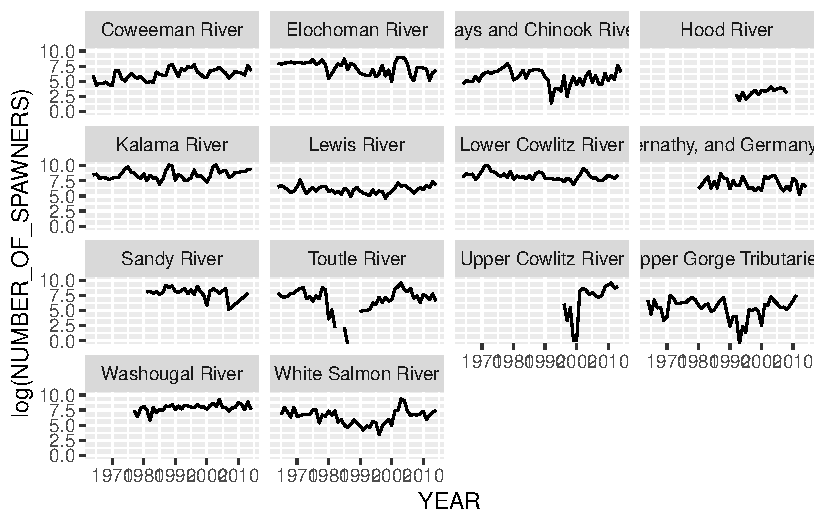
\includegraphics{text/figures_files/figure-pdf/fig-salmon-1.pdf}

}

\caption{\label{fig-salmon}Plot of the data}

\end{figure}

\bookmarksetup{startatroot}

\hypertarget{conclusion}{%
\chapter{Conclusion}\label{conclusion}}

Lorem ipsum dolor sit amet, consectetur adipiscing elit. Nam commodo sit
amet nibh non molestie. Maecenas hendrerit nisl velit, a condimentum
enim lobortis sit amet. Ut vitae nunc sed mauris condimentum fermentum.
Mauris pellentesque nec neque id elementum. Suspendisse a quam aliquam,
facilisis urna venenatis, malesuada diam. Pellentesque in fringilla
orci. Cras sed purus urna. Ut pharetra enim ut ligula egestas mattis.

Phasellus non diam posuere, laoreet velit sed, egestas felis. Etiam eget
neque in tellus lacinia tincidunt. Pellentesque scelerisque odio velit,
nec fringilla nibh iaculis non. Aenean sit amet nulla ipsum. Cras felis
lacus, pulvinar ac nisi et, convallis pulvinar turpis. Morbi non nibh
lacus. Morbi vitae lorem massa. Sed ut turpis vel felis posuere commodo
lacinia ac mi. Donec finibus lectus sit amet elit finibus, vitae rhoncus
ligula tincidunt. Phasellus vitae blandit lacus. Integer sed nisl
fermentum, pulvinar mauris in, posuere enim. Proin sit amet semper urna.
Vivamus aliquet rutrum diam ac luctus.

Quisque in nibh sit amet nunc mollis porttitor quis et mauris. Sed non
condimentum leo, ac condimentum est. Duis ac venenatis nulla, et aliquet
elit. Suspendisse potenti. Duis mollis dui at semper luctus. Maecenas
euismod finibus condimentum. Fusce vitae gravida massa. Mauris metus
est, pretium non semper vel, dictum vel augue.

Curabitur tempus, leo quis volutpat rhoncus, turpis elit vehicula dolor,
id tincidunt augue nunc at enim. In vel enim mattis, varius orci at,
tempus ante. Morbi massa elit, pharetra ac libero at, porta tempus quam.
Ut fringilla, tortor ac tristique euismod, magna felis vestibulum
turpis, quis congue mauris leo nec felis. Aliquam viverra et nibh ut
blandit. Praesent sed luctus odio. Pellentesque finibus velit dolor.
Morbi ac pulvinar ex, id dapibus eros. Cras interdum arcu viverra auctor
tristique. Suspendisse venenatis volutpat ultricies.

Donec bibendum pharetra arcu vitae porttitor. Morbi ac quam nunc. Ut
cursus dolor a mauris aliquet vulputate. Morbi elementum ullamcorper
augue, et tincidunt libero facilisis posuere. Nam congue velit non elit
sollicitudin aliquet. Donec lobortis nunc ligula, id sollicitudin erat
rhoncus cursus. Ut egestas orci libero, eu malesuada ex sollicitudin
sed. Sed ornare nunc eget massa scelerisque, nec egestas nulla commodo.
Pellentesque efficitur accumsan ullamcorper. Nulla facilisi. Maecenas
tristique luctus malesuada. Phasellus id enim maximus, tempus tellus eu,
dignissim sapien. Integer et mauris in lectus condimentum pellentesque
non a felis.

\bookmarksetup{startatroot}

\hypertarget{references}{%
\chapter*{References}\label{references}}
\addcontentsline{toc}{chapter}{References}

\markboth{References}{References}

\hypertarget{refs}{}
\begin{CSLReferences}{0}{0}
\end{CSLReferences}

\appendix
\addcontentsline{toc}{part}{Appendices}

\hypertarget{crchum.csv}{%
\chapter{CRchum.csv}\label{crchum.csv}}

\hypertarget{tbl-appA1}{}
\begin{table}
\caption{\label{tbl-appA1}Spawners and fracwild from Grays \& Chinook Rs. for 2001 to 2010. }\tabularnewline

\centering
\begin{tabular}[t]{rrr}
\toprule
Year & Spawners & Fracwild\\
\midrule
2001 & 4742 & 0.895\\
2002 & 11713 & 0.896\\
2003 & 16669 & 0.933\\
2004 & 13716 & 0.959\\
2005 & 4204 & 0.903\\
\addlinespace
2006 & 6605 & 0.933\\
2007 & 3999 & 0.955\\
2008 & 2608 & 0.921\\
2009 & 2876 & 0.965\\
2010 & 6380 & 0.953\\
\bottomrule
\multicolumn{3}{l}{\rule{0pt}{1em}\textit{Note: }}\\
\multicolumn{3}{l}{\rule{0pt}{1em}kable}\\
\multicolumn{3}{l}{\textsuperscript{} ** data file: CRchum.csv mod}\\
\multicolumn{3}{l}{date: Sat Aug 13 16:58:50}\\
\multicolumn{3}{l}{2022 -0600}\\
\multicolumn{3}{l}{\textsuperscript{} * These spawner counts are}\\
\multicolumn{3}{l}{from river redd surveys.}\\
\end{tabular}
\end{table}

\newpage

\hypertarget{tbl-appA2}{}
\begin{table}
\caption{\label{tbl-appA2}Spawners and fracwild from Washougal R. for 2005 to 2010. }\tabularnewline

\centering
\begin{tabular}[t]{lrrr}
\toprule
  & Year & Spawners & Fracwild\\
\midrule
19 & 2005 & 923 & 0.977\\
20 & 2006 & 869 & -99.000\\
21 & 2007 & 576 & -99.000\\
22 & 2008 & 644 & -99.000\\
23 & 2009 & 1154 & 0.969\\
\addlinespace
24 & 2010 & 2148 & -99.000\\
\bottomrule
\multicolumn{4}{l}{\rule{0pt}{1em}\textit{Note: }}\\
\multicolumn{4}{l}{\rule{0pt}{1em}kable}\\
\multicolumn{4}{l}{\textsuperscript{} ** data file: CRchum.csv mod date:}\\
\multicolumn{4}{l}{Sat Aug 13 16:58:50 2022 -0600}\\
\multicolumn{4}{l}{\textsuperscript{} * These spawner counts are from}\\
\multicolumn{4}{l}{river redd surveys.}\\
\end{tabular}
\end{table}

\newpage

\hypertarget{hcchum.csv}{%
\chapter{HCchum.csv}\label{hcchum.csv}}

\hypertarget{tbl-appB1}{}
\begin{table}
\caption{\label{tbl-appB1}Spawners and fracwild from Strait of Juan de Fuca for 2000 to 2010. }\tabularnewline

\centering
\begin{tabular}[t]{lrrr}
\toprule
  & Year & Spawners & Fracwild\\
\midrule
30 & 2000 & 801 & 0.49\\
31 & 2001 & 3733 & 0.36\\
32 & 2002 & 6791 & 0.61\\
33 & 2003 & 6752 & 0.62\\
34 & 2004 & 9280 & 0.60\\
\addlinespace
35 & 2005 & 9619 & 0.62\\
36 & 2006 & 8181 & 0.82\\
37 & 2007 & 3219 & 0.93\\
38 & 2008 & 3449 & 0.86\\
39 & 2009 & 5029 & 0.59\\
\addlinespace
40 & 2010 & 9179 & 0.65\\
\bottomrule
\multicolumn{4}{l}{\rule{0pt}{1em}\textit{Note: }}\\
\multicolumn{4}{l}{\rule{0pt}{1em}kable}\\
\multicolumn{4}{l}{\textsuperscript{} ** data file: HCchum.csv mod date:}\\
\multicolumn{4}{l}{Sat Aug 13 16:58:50 2022 -0600}\\
\multicolumn{4}{l}{\textsuperscript{} * These spawner counts are from}\\
\multicolumn{4}{l}{river redd surveys.}\\
\end{tabular}
\end{table}

\newpage

\hypertarget{tbl-appB2}{}
\begin{table}
\caption{\label{tbl-appB2}Spawners and fracwild from Hood Canal for 2000 to 2010. }\tabularnewline

\centering
\begin{tabular}[t]{lrrr}
\toprule
  & Year & Spawners & Fracwild\\
\midrule
82 & 2000 & 7987 & 0.67\\
83 & 2001 & 11491 & 0.60\\
84 & 2002 & 10818 & 0.60\\
85 & 2003 & 35173 & 0.77\\
86 & 2004 & 69565 & 0.86\\
\addlinespace
87 & 2005 & 15311 & 0.72\\
88 & 2006 & 26418 & 0.80\\
89 & 2007 & 10539 & 0.87\\
90 & 2008 & 15112 & 0.88\\
91 & 2009 & 7236 & 0.89\\
\addlinespace
92 & 2010 & 12533 & 0.91\\
\bottomrule
\multicolumn{4}{l}{\rule{0pt}{1em}\textit{Note: }}\\
\multicolumn{4}{l}{\rule{0pt}{1em}kable}\\
\multicolumn{4}{l}{\textsuperscript{} ** data file: HCchum.csv mod date:}\\
\multicolumn{4}{l}{Sat Aug 13 16:58:50 2022 -0600}\\
\multicolumn{4}{l}{\textsuperscript{} * These spawner counts are from}\\
\multicolumn{4}{l}{river redd surveys.}\\
\end{tabular}
\end{table}

\newpage


\backmatter

\end{document}
